\documentclass[11pt]{article}
\usepackage[margin=1in]{geometry}
\usepackage{graphicx,booktabs,amsmath,hyperref}
\title{GLAM on the offline $\beta(\rho)$ curve:\\ single-anchor run (r24) versus multi-anchor run (r24m)}
\author{Aidan Gettemy}
\date{October 29, 2026}
\begin{document}
\maketitle

\section{Summary}
Both runs used 24 chains (one per core), $\sigma_{\rm conc}=0.002$, $\sigma_{\rm dp}=0.004$, a target acceptance of 0.25, and 40\,000 iterations (adaptation in the first 14\,000). They differ only in how the chains are restarted at the stage exchanges.
\begin{itemize}
\item \textbf{r24:} one anchor, namely the best state; every chain restarts near it (scale 0.01).
\item \textbf{r24m:} open archive (no maximum number of anchors, no minimum distance, quality tolerance 50 in $\Phi$), with 25\% of the chains restarting from the exploit role, 25\% from frontier and 50\% from explore (restart scales 0.01, 0.03, 0.08).
\end{itemize}
\textbf{Result.} The multi-anchor run did not improve on the single-anchor run. It ended with a higher $\Phi$ (best anchor 890 versus 738), a higher concentration misfit, and a slightly lower field correlation. The archive grew to several hundred anchors, but their effective rank fell to 1.8: the anchors lie along one descent path, not at distinct modes. The posterior spread is slightly wider in r24m (mean sd 0.31 versus 0.27 in $\ln K$), yet the 1$\sigma$ and 2$\sigma$ coverages remain far below nominal in both runs.

\section{Fit and field comparison}
\begin{table}[h]\centering
\begin{tabular}{lrr}\toprule
 & r24 & r24m \\ \midrule
Best anchor $\Phi$ at the end (iteration 39\,896) & 738 & 890 \\
Best sampled state $\Phi$ & 731 & --- \\
RE$_{\rm conc}$, median over tail / chains & 0.0826 & 0.0916 \\
RE$_{\rm conc}$, 5--95\% & 0.077--0.094 & 0.086--0.099 \\
RE$_{\rm dp}$, median & 0.00235 & 0.00228 \\
Tail acceptance, global / local (mean over chains) & 0.219 / 0.219 & 0.218 / 0.223 \\
\midrule
Field corr., best sample & 0.650 & 0.589 \\
Field corr., posterior mean & 0.648 & 0.609 \\
RMSE ($\ln K$), best sample & 0.779 & 0.837 \\
RMSE ($\ln K$), posterior mean & 0.765 & 0.794 \\
Mean level of $\ln K$, best sample vs.\ reference ($-29.9996$) & $-29.990$ & $-29.985$ \\
Coverage 1$\sigma$ / 2$\sigma$ & 0.277 / 0.516 & 0.303 / 0.544 \\
rms $z$-score & 3.37 & 3.29 \\
Mean posterior sd of $\ln K$ & 0.274 & 0.305 \\ \bottomrule
\end{tabular}
\caption{Fit and field statistics from \texttt{diagnostics.json} and \texttt{field\_comparison.json} (tail after iteration 14\,000). The reference field has sd$(\ln K)=0.966$. The best sample of r24m was not exported, so its $\Phi$ is not listed.}
\end{table}
The pressure-drop fit is the same in both runs. The ordering of the two runs on the concentration data, on the field correlation and on RMSE agrees across every row of the table, but each is a single run, so differences of this size could also come from the random seed.
The best state of r24 has $\rho=0.884$, $\beta=9.62\times10^{-14}$ (2.6\% below $\beta_{\rm true}=9.87\times10^{-14}$) and a pressure drop of 3308.2~Pa against the data value 3314.7~Pa.

\begin{figure}[h]\centering
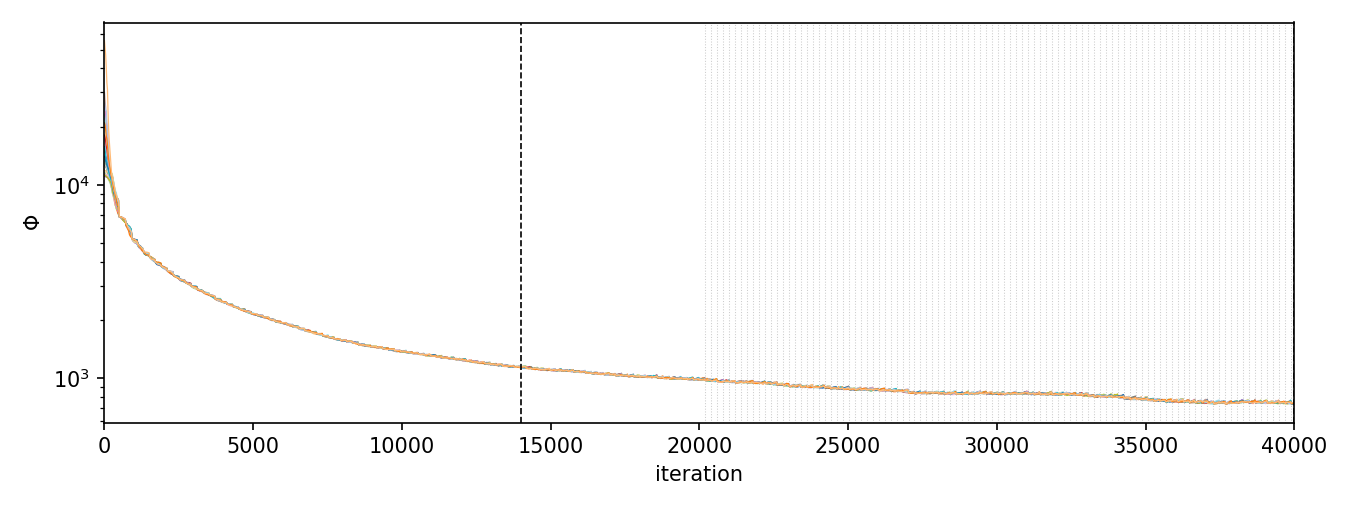
\includegraphics[width=0.49\textwidth]{fig_traces_phi_r24.png}\hfill
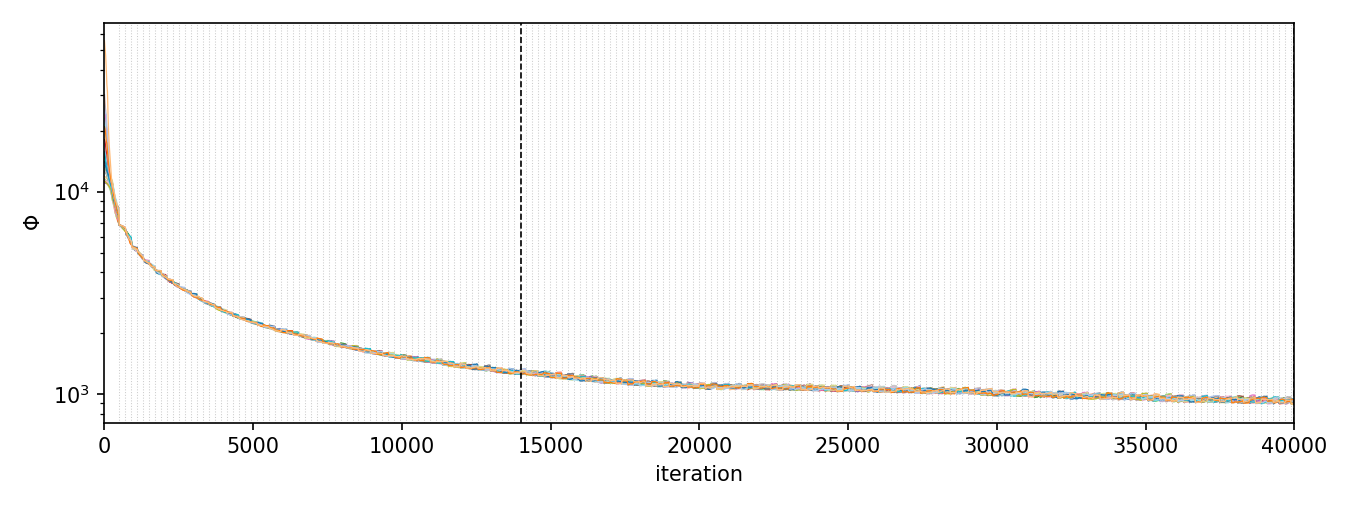
\includegraphics[width=0.49\textwidth]{fig_traces_phi_r24m.png}
\caption{$\Phi$ of all 24 chains versus iteration (log axis). Left: r24; right: r24m. Dotted lines mark exchanges (r24 shows them only for the last continuation; the dashed line is the end of adaptation). In both runs the 24 chains lie on one curve.}
\end{figure}

\section{Convergence diagnostics}
The multivariate PSRF is near one in both runs (Table~2), but it is not informative here: the chains restart from the same state at every exchange, so they cannot disagree.
\begin{table}[h]\centering
\begin{tabular}{lrrrr}\toprule
 & \multicolumn{2}{c}{final MPSRF} & \multicolumn{2}{c}{iteration at level 1.2}\\
 & r24 & r24m & r24 & r24m \\ \midrule
$\rho$ (whitened) & 1.000 & 1.003 & 15\,200 & 15\,200\\
first 100 coordinates & 1.015 & 1.030 & 16\,392 & 17\,824\\
block 0 (500 dims) & 1.069 & 1.107 & 24\,163 & 27\,890\\
max per-coordinate PSRF & 1.001 & 1.007 & & \\ \bottomrule
\end{tabular}
\caption{MPSRF from iteration 14\,000 (2600 thinned samples).}
\end{table}

\section{Anchor history}
The r24 table covers only the last continuation (iterations 20\,198--39\,896, 99 exchanges), where there was always one anchor. The r24m table covers the whole run (197 exchanges).
\begin{figure}[h]\centering
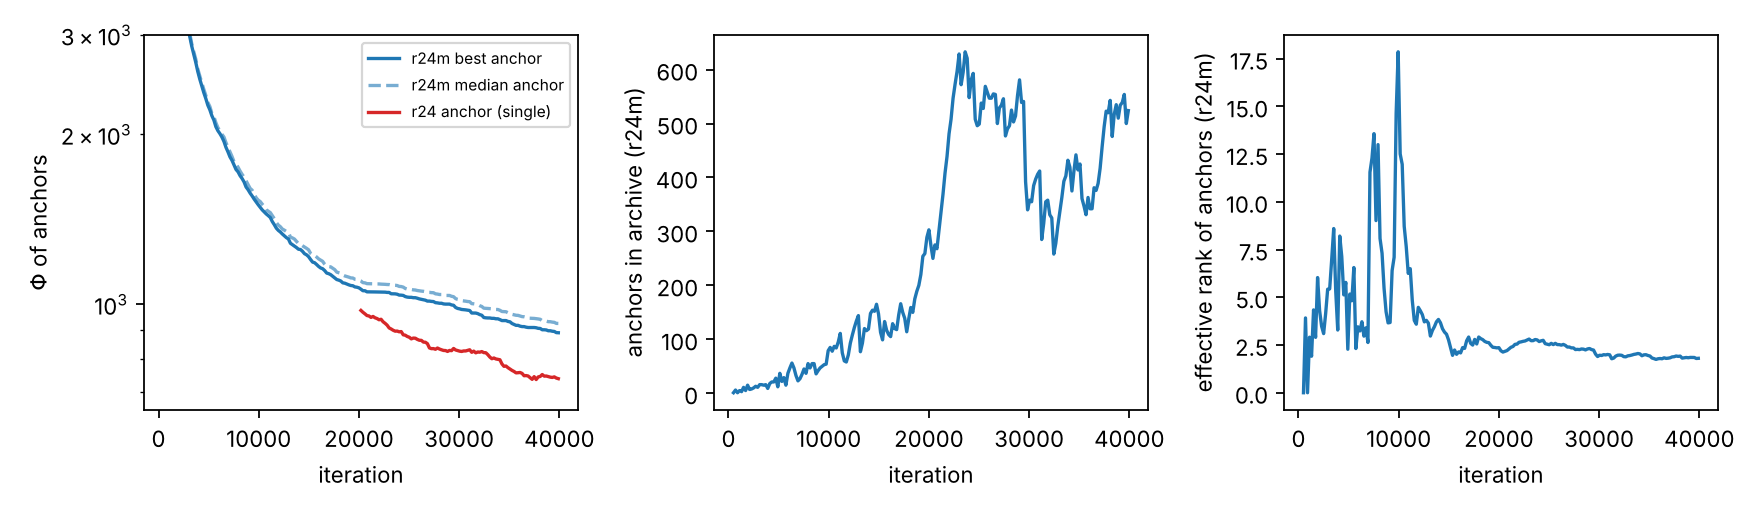
\includegraphics[width=\textwidth]{fig_exchange.png}
\caption{Left: $\Phi$ of the best and median anchor of r24m, and the single anchor of r24 (continuation only). Middle: archive size in r24m. Right: effective rank of the r24m anchors.}
\end{figure}
\begin{itemize}
\item \textbf{Archive size.} It grows from 1 to 29, 87 and 133 anchors by iteration 15\,575, then fluctuates between roughly 270 and 570 (maximum 633). It falls at times because the best $\Phi$ keeps decreasing and the quality tolerance (50) removes older anchors.
\item \textbf{Rebuild cost.} The rebuild takes about 10~s on average and at most 42~s. In total it is 34~min per rank over a run of many hours.
\item \textbf{Diversity.} The median distance between anchors stays near 23 (one exchange has 78), and the effective rank falls from 5--9 early on to 1.8 at the end. The spread of $\Phi$ among anchors is about 35 (median minus best), set by the quality tolerance.
\item \textbf{Roles.} The best anchor comes from the exploit role at every exchange. Every restart was accepted in every role, and the radii were never reduced (0.025 frontier, 0.08 explore), so the $\Phi$ acceptance criterion never bound. The explore role could have been given a much larger radius.
\end{itemize}

\section{Descent compared at equal iteration}
\begin{table}[h]\centering
\begin{tabular}{rrr}\toprule
iteration (r24 / r24m) & r24 $\Phi$ & r24m best-anchor $\Phi$ \\ \midrule
20\,198 / 20\,600 & 975 & 1056 \\
25\,223 / 25\,625 & 868 & 1027 \\
30\,248 / 30\,650 & 825 & 977 \\
35\,273 / 35\,675 & 763 & 917 \\
39\,896 / 39\,896 & 738 & 890 \\ \bottomrule
\end{tabular}
\caption{Best-anchor $\Phi$ at matching exchanges.}
\end{table}
Between iterations 20\,000 and 40\,000 r24 lowered $\Phi$ by 24\%, r24m by 16\%. Neither run has flattened: both are still descending at 40\,000 iterations, so neither has reached the equilibrium level (floor 7.6 plus about half the number of data-constrained parameters).

\section{Interpretation and caveats}
\begin{itemize}
\item \textbf{Why r24m is slower (hypothesis, not tested).} In r24 all chains restart at the best state each time. In r24m only the 25\% exploit chains do; the frontier and explore chains restart from other anchors, which have $\Phi$ up to 50 above the best. The restarts thus dilute the progress along the descent path. The tail of the $\Phi$ traces in Figure~1 shows slightly more chain-to-chain scatter in r24m.
\item \textbf{Confounds.} Each configuration was run once. r24 ran in two pieces (an initial run and one continuation), r24m in one run with a different stage and exchange schedule (an exchange about every 200 iterations throughout), so part of the difference may come from the schedule or the seed, not from the archive.
\item \textbf{Diversity in the wrong directions.} The data constrain few directions of $\theta$. The archive diversity is in the unconstrained ones, which do not change $\Phi$ or $\rho$. This matches the single trace of $\rho$ and $\Phi$ across the chains.
\item \textbf{Posterior calibration.} Coverage of 28--30\% (1$\sigma$) and 52--54\% (2$\sigma$) with rms $z\approx3.3$ shows the sampled spread is too narrow in both runs. This is expected for chains that have not left the descent phase, so it is not evidence about the model.
\end{itemize}

\section{Suggested next steps}
\begin{enumerate}
\item Raise the explore radius (0.08 to about 0.3) and the frontier radius (0.025 to about 0.1), so that the $\Phi$ tolerance can bind. Check the acceptance fractions in the exchange table.
\item Address the slow descent itself, which limits both runs: a warm start (ensemble smoother), or a coarse-to-fine ramp of the modes.
\item Export the best sample of r24m (\texttt{export\_glam\_fields.py}) and add it to Table~1.
\item Rerun r24 with the exchange schedule of r24m and a different seed, to separate the effect of the restart scheme from the schedule and the seed.
\end{enumerate}

\end{document}
